%\renewcommand{\refname}{Bibliografía}
%\bibliographystyle{ieeetr}
%\bibliography{referencias}

%%%%%%%%%%%%%%%%%%%%%%%%%%%%%%%%%%%
%%%%%%%%%%%%%%%%%%%%%%%%%%%%%%%%%%%%
%%%%%%%%%%%%%%%%%%%%%%%%%%%%%%%%%%%

\begin{comment}

\input{Ejercicio1.tex}







\blfootnote{\textbf{\textit{Nota: }}Excelente formato de práctica, sin duda.}



\begin{Graphs}[H]
\centering
\includegraphics[scale=1]{./images/plotbat.eps} 
\caption{Símbolo de Batman.}
\label{g1}
\end{Graphs}



\begin{esq}[H]
\centering
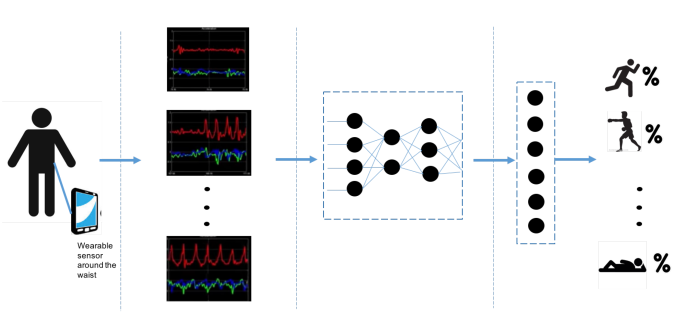
\includegraphics[scale=1]{./images/1.eps} 
\caption{Sistema eléctrico procesado en TINA-TI.}
\label{e1}
\end{esq}




\begin{figure}[H]
\centering
\includegraphics[scale=1]{./images/a20.eps} 
\caption{Pares ordenados para h = 2.}
\label{f1}
\end{figure}




\lstset{language=C, breaklines=true, basicstyle=\footnotesize}
\begin{lstlisting}[frame=single,caption={Código del método de la secante},label={c1}, captionpos=b]

línea 1
\end{lstlisting}
\end{comment}




\begin{table}[H]
  \centering
    \begin{tabular}{|l|l|}
    \hline
    $V_{ref}$   & $4.2\; V$ \bigstrut\\
    \hline
    $R$    & $322\; \Omega$ \bigstrut\\
    \hline
    $C$     & $0.31 \;\mu F$ \bigstrut\\
    \hline
    \end{tabular}%
     \caption{Valores asignados}
  \label{tab:addlabel}%
\end{table}%



\section{Apéndices}
\includepdf[pages=2-8]{./files/NTE093B.pdf} 
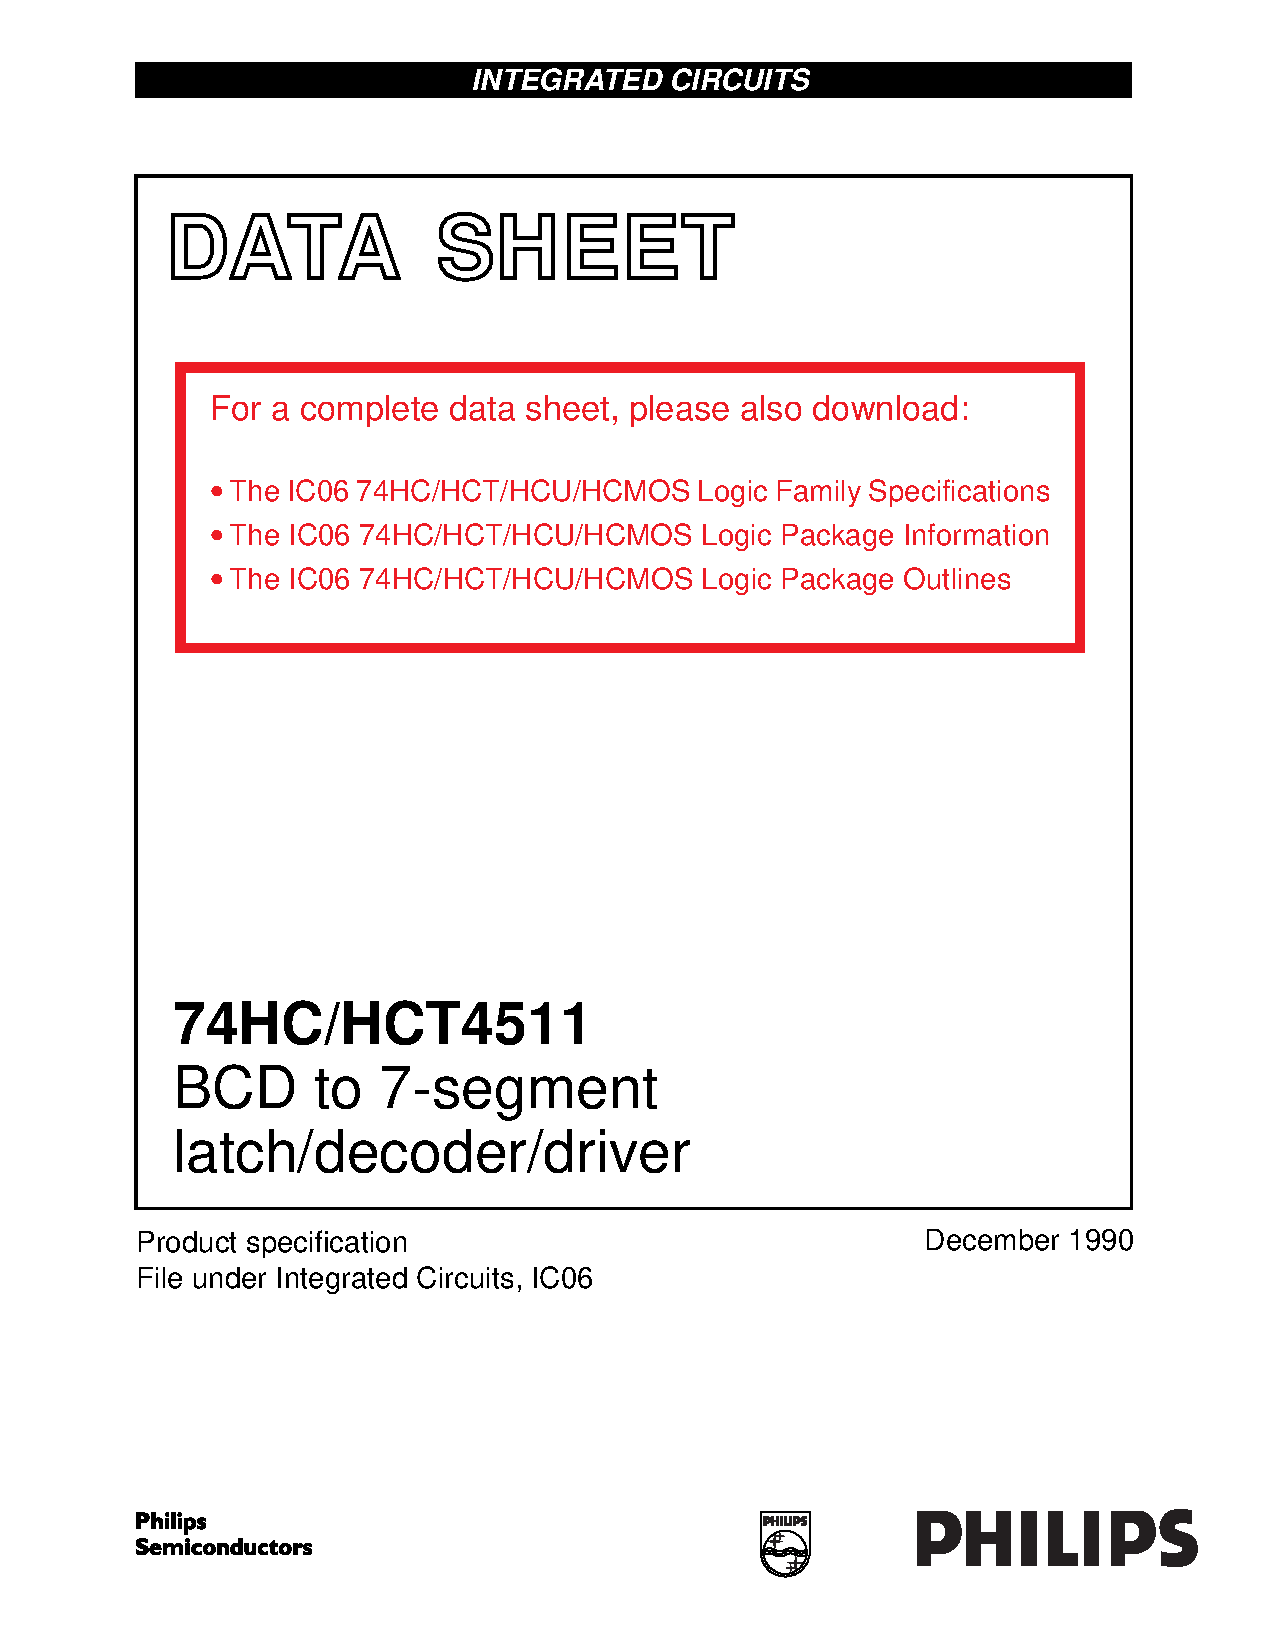
\includepdf[pages=-]{./files/bcd.pdf}



\cite{porter2008cinco}\blfootnote{\textbf{\textit{Nota: }}Excelente formato de práctica, sin duda.}




\begin{minted}{verilog}
codigo linea 1
\end{minted}


%%%%%%%%%%%%%%%%%%%%%%%%%%%%%%%%%%%%%
%%%%%%%%%%%%%%%%%%%%%%%%%%%%%%%%%%%%%
%%%%%%%%%%%%%%%%%%%%%%%%%%%%%%%%%%%%%